\chapter{Virtual Spaces}


Over the past twenty years, the prospect of visiting a virtual world different from our own world has moved from being strictly the domain of imagination to being widely accessible. What started as worlds accessed through typed commands and presented as text have evolved into rich graphical and sensorial experiences that became rapidly accessible to mass audiences. The argument for virtual worlds has always had a revolutionary tone. Virtual worlds might, for example, suppress the prejudices of offline society by hiding identity information, breaking down the boundaries of distance, and making experiences broadly accessible that might not otherwise be feasible. Perhaps we could even build a new virtual society, one that is better than our own. These utopian visions are attractive precisely because the urge to grow beyond the confines of everyday experience is so strong.

This vision was so attractive that in the mid 2000's the market research firm Gartner famously predicted in 2007 that by the end of 2011, ``80 percent of active Internet users (and Fortune 500 enterprises) will have a `second life', but not necessarily in \emph{Second Life}.'' \citep{Anonymous:2007wz}. This has not come to pass. Linden Lab has stopped publishing public usage data, but it is clear by comparing its cultural impact to systems like \emph{Facebook}, \emph{Twitter}, and \emph{YouTube} that \emph{Second Life} has been almost completely eclipsed in the public imagination by other types of mediated social experiences. Despite this shift, it is still productive to attend to this period where virtual worlds were viewed as strong potential venues for mediated social interaction. What attracted us to these experiences in the first place? Why did these experiences ultimately fail to catch people's imaginations? Are there aspects of ``virtual'' experiences that were left behind in the shift away from a ``virtual'' approach that might be valuable components of more modern experiences? Why did the reality of accessible virtual worlds fail to live up to their revolutionary, utopian promise?

In this chapter I will address these questions through an analysis of the properties of virtuality and a pair of design projects: \emph{Information Spaces} and \emph{Presentation Spaces}. Although these projects do not exemplify the best sorts of \emph{in situ} research, they serve as conceptual arguments about how we might think about designing virtual experiences that take advantage of what virtuality offers designers that is missing in other approaches to mediated interaction. This is in contrast to much of the design work in virtual worlds in this period that focused instead on replicating the forms of offline experiences and expecting them to have the same properties when transplanted into a virtual context.

Although in its specifics this argument is perhaps a little dated and unlikely to apply directly in the future (barring a resurgence of virtual world design), it can be seen also as an argument for how to do a close reading of the properties of a platform and letting those properties guide a design that is closely adapted to its tools. Considering virtual worlds in this detail helps highlight some of the taken-for-granted assumptions about non-virtual design.

In a larger sense, a deep discussion of virtuality will also demonstrate how the core research themes of this thesis--grounding, non-verbal actions, and attention--operate in an unfamiliar context. Although readers might be unfamiliar with operating in a virtual world environment, this unfamiliarity will help address these research themes without preconceptions.

I open this chapter with a discussion of what precisely defines a ``virtual world'', focusing on the distinction between spatiality and dimensionality. 


% TODO this isn't actually how I open, fix this.




I will defer an analysis of why this might have happened for later in this chapter, but 


As with many technology trends, there is a sort of pendulum that swings between different design strategies. Our earliest mediated social experiences (like email and chat) were primarily text-based media. 



This chapter explores some of my early work in the virtual world space and draw comparisons between 


\section{Characterizing Virtual Worlds}

Although there is no single definitive typology of virtual worlds (though there are many examples, e.g. \citep{Koster:2007wg}), there are a few general categories that are important to properly describe the kind of worlds that this thesis is concerned with.\sidenote{This section draws heavily from \citep{Harry:2008vx}.}

The two major axes on which virtual worlds can be organized (as proposed by \citet{Bartle:2003up} are agency (which Bartle calls `change') and persistence. Agency is a broad term that is the set of things that someone can do in a world. Agency can be thought of as the interface that you have onto the world. For example, the agency of players in a chess game is limited. When it's their turn they can move their own pieces in certain prescribed ways. Moving pieces is the agency players have in the chess game. In virtual worlds, agency becomes a bit more elaborate and includes movement, avatar customization, communication, object creation, etc. Different worlds have different sets of actions that an avatar can do, and I describe them as having different kinds of agency.

Persistence is the ability of the world to remember events that change something about the world. For example, if you create an object in a persistent virtual world you can expect that the object will be there when you return. This is in contrast to worlds where changes aren't saved for very long. Multiplayer first person shooter games are a good example of this---you interact with a rich three-dimensional world and might change it by dropping weapons, causing explosions that change the appearance of part of it, or by destroying certain objects in the environment. None of those changes will remain in that world the next time you play, though. It will be wiped clean and you'll have a fresh copy of the original space. These spaces often even revert to their original state after a few minutes: bodies disappear, dropped weapons fade, and explosion marks are removed. 

Certainly, these axes are not perfectly distinct (worlds with limited agency often have low persistence as well), but they serve as good organizing principles. For the most part, modern virtual worlds have high levels of agency but relatively low levels of persistence. In \emph{World of Warcraft} for instance, players can kill monsters in the world, but the monsters will always reappear a few minutes later. There are virtually no actions players can take that modify any aspect of the world apart from killing computer controlled characters. Rich agency exists almost entirely in the relationships between players and the organizations they form. Worlds like this have proven to be commercial successes because they are more resistant to disruptive behavior aimed at degrading other players' experiences, but they also rule out many of the interesting opportunities that virtual spaces offer over physical spaces.

The best recent example of a world that offers that kind of rich agency and persistence is \emph{Second Life}, a world developed by Linden Lab. \emph{Second Life} is a free application that connects to a single monolithic ``Grid'' of \emph{Second Life} servers that provide a mostly continuous (flat) virtual space in which avatars can own land and items, build clothing, buildings, or vehicles, and embed behavioral scripts in their creations. The world also provides an economic system with its own currency system (the Linden Dollar, L\$), which is exchangeable at a fixed rate for US Dollars on a currency exchange that Linden Lab manages. The community that has arisen around \emph{Second Life} is extraordinarily diverse and rich, but an in depth discussion of its dynamics is beyond the scope of this chapter. There are a number of books that describe the history and culture of \emph{Second Life}, which provide a good introduction to that topic, however. \citep{Au:2008va, Ludlow:2007uu} For my purposes, \emph{Second Life} is critical as an example of a world in which avatars have a considerable amount of control over the design of environments, and so \emph{Second Life} has been instrumental in developing an intuition for how virtual spaces influence the behavior of people in them. It has also been useful as a platform for exploring the design space of algorithmic architecture. For much of this chapter, I will turn to \emph{Second Life} as a source of inspiration, as well as to draw comparisons between the general model for virtual architecture that I explore in this thesis and the model that \emph{Second Life} embodies.

The following sections lay out the pieces of what might make something feel like a world. There is not clear set of necessary and sufficient conditions for world-ness. Instead, these sections introduce a series of concepts that all lend-themselves to fostering a sense of world-ness. These concepts are Representation, Spatiality, and Presence. 

\subsection{Representation and Function}
Specific features of both physical spaces and virtual spaces can be thought of as serving symbolic and functional purposes. As virtual spaces were first being conceived it was not obvious that they would draw their symbolism heavily from physical spaces \citep{Novak:1991ue}. Novak would no doubt be surprised to see how familiar the design elements of can be. In the free-form world \emph{Second Life}, for instance, there are countless recreations of both specific architectural landmarks as well as buildings that ape familiar architectural styles. Furthermore, those buildings are filled with rooms furnished in a way that would not stand out in the least from their real world analogs. Why is it that, free of the natural laws of the physical world, so much of virtual world design is concerned with recreating familiar physical spaces?

This focus on familiar representations serves a number of important social roles. First, it functions much like the identity signals do in physical fashions. Although choosing and furnishing a virtual house is substantially less costly than its physical analog, it is still a strong demonstration of taste that helps visitors to virtual spaces understand something about the person who assembled them, much like a personal homepage or profile page might on the Web. And though the price of virtual items may be substantially less than the physical artifact it mimics, virtual economies usually have some sense of relative value that allow these items to also function as signals of wealth.

\begin{figure*}[t]
	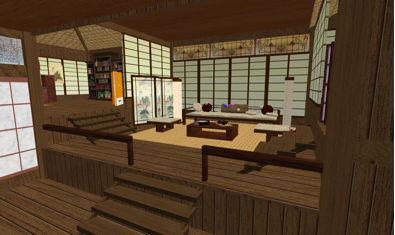
\includegraphics{figures/asian_home.png}
	\caption{A \emph{Second Life} home decorated in an Asian style.}
	\label{fig:asian_home}
\end{figure*}

The second important social role is in building spaces that contextualize behavior. Visitors to virtual worlds are forced to reform their notions of socially acceptable behavior in virtual spaces. It is substantially easier to make meaning from a virtual space built to look like something familiar than something abstract. In this way, avatars in virtual spaces can reasonably expect that spaces that look like virtual museums, dance clubs, meeting rooms or houses should be used for virtual analogs of what one might do in their offline equivalent. This argument is analogous to Norman's, with respect to the design of interactions with physical objects \citep{Norman:2002tv}. He describes how physical objects use metaphors to demonstrate affordances. Metaphors imply a conceptual model that makes it easier for people to make deductions about what how their interactions with the system will affect it. In a very similar way, literal representations in virtual architecture serve as behavioral affordances. They use architectural metaphors to imply what the social model of the space should be. 

Although literal representational techniques serve effectively as identity signals and behavioral affordances, this does not mean that they are the only way to do effective design work in virtual worlds. Indeed, the work in this chapter will try to demonstrate an alternate approach.

I will describe spaces which not just look different and imply that different behaviors are expected but spaces that actually have different functional affordances that make certain activities more or less effective in a particular space. Functional affordances are those that are not simply based on what the space looks like, but what aspects of the world that are algorithmic and reactive in some way. We should treat virtual space as a new medium that has its own strengths and weaknesses instead of trying to create the experience of ``being there.'' This distinction is best understood through analogy to how symbolism and function interplay in two kinds of physical spaces: cathedrals and nightclubs.

\begin{figure*}[t]
	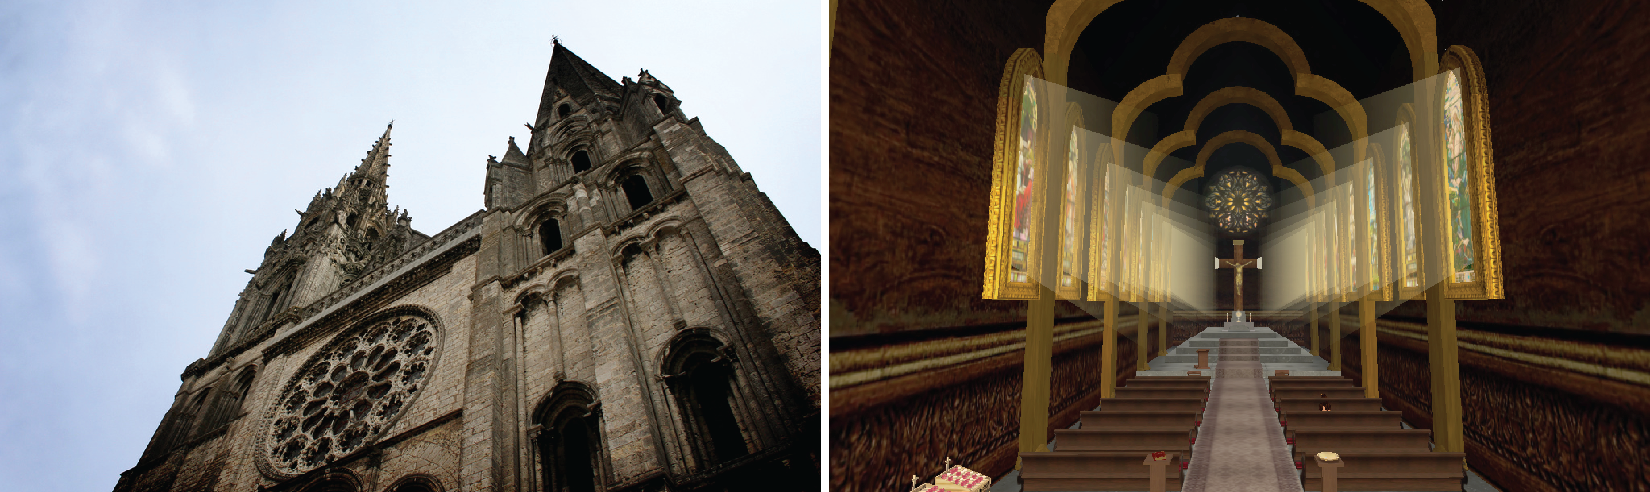
\includegraphics{figures/cathedral_comparison.png}
	\caption{Left: Photo of a cathedral, courtesy of flickr user glynnis. Right: Screenshot of a cathedral in \emph{Second Life}.}
	\label{fig:cathedral_comparison}
\end{figure*}

The form of a classical cathedral is rich with religious symbolism that informs the overall structure of the building, detailed adornments, lighting, and scale. It also has certain functional affordances. The space is designed such that a speaker at the podium can be easily seen and heard by the people in the pews. This also means that the whole congregation will easily hear any noises from the pews. This encourages parishioners to be quiet, and re-enforces the power dynamics inherent to the church; visitors are not there to interact with each other.

Nightclubs use acoustics and lighting to create a very different kind of space. Although the precise form of clubs varies, the functional aspects of clubs are often quite similar. Loud music makes it hard to hear people far away, which both forces people to be close together to talk and makes it hard to be overheard. In this environment, it is easy to have intimate conversations. Low lighting makes it difficult to see people, hear them, and identify them. This creates a situation in which people must fill in information about each other because the environment makes that information hard to get. Darkness and candlelight in a cathedral would have a different effect---the functional and cultural/symbolic meanings are interwoven.  The nightclub is known to be about hedonism and escape; the cathedral, for the believer, about spiritual, solemn, and perhaps frightening/awe-inspiring experience.

Lighting and acoustics are two aspects of what I call ``functional'' aspects of space. They operate mostly independently of how a space looks (that is to say two spaces could look the same but have different acoustics) and both respond to people's actions in the space as well as mold those actions. These two examples demonstrate how the functional side of spaces has a big impact on what kind of activities make sense in them. You would not, for instance, try to hold a business meeting in a nightclub or hold small group discussions in a cathedral. Yet virtual spaces very rarely have this kind of adaptability to their designed purposes. You could, in a world like \emph{Second Life}  hold a business meeting in a virtual night club with no particular ill effects. It would be a strange juxtaposition, but the location would be only a visual distraction, not a major impediment to having a conversation. The heart of this chapter is to show how building virtual spaces that exhibit some of these same sorts of properties might create compelling virtual experiences that are competitive with non-virtual interfaces.

\begin{figure*}[t]
	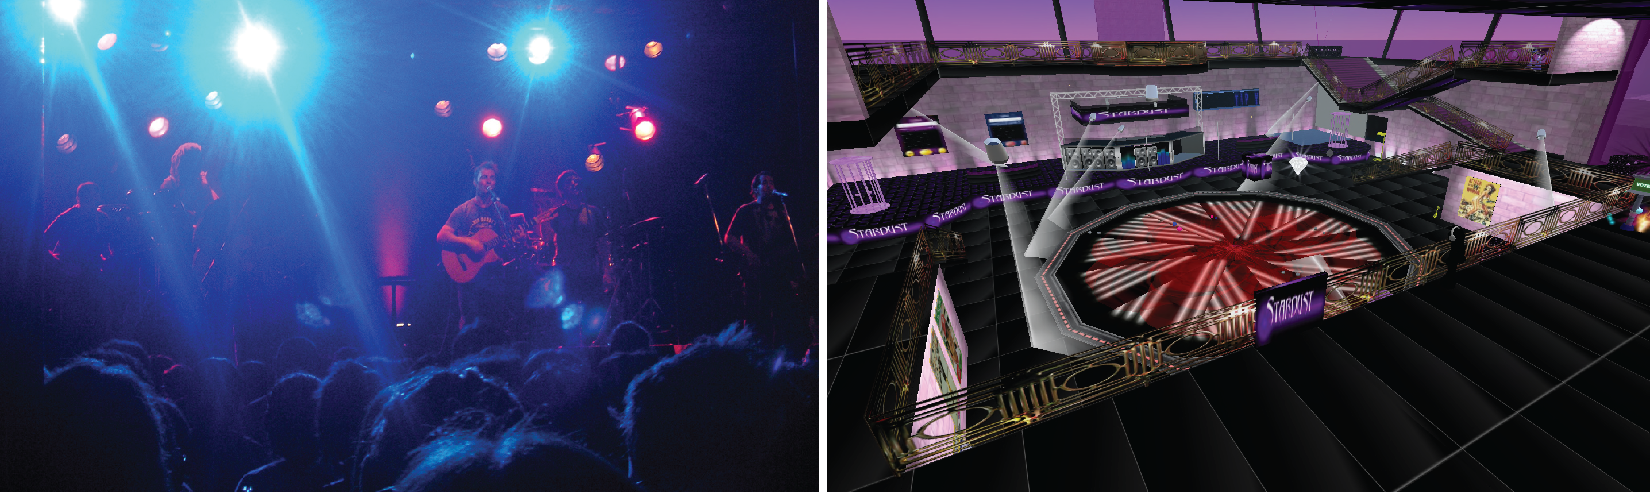
\includegraphics{figures/club_comparison.png}
	\caption{Left: Photo of a nightclub. Right: An empty nightclub in \emph{Second Life}.}
	\label{fig:nightclub_comparison}
\end{figure*}

\subsection{Dimensionality and Spatiality}

It's difficult to pin down exactly what makes a virtual world a world. In the previous section we draw the distinctions of agency and persistence from the literature. These are useful for distinguishing between different sorts of world, but are not sufficient to distinguish worlds from non-worlds. Another attractive potential to draw a distinction between worlds and non-worlds might be a certain immersive representation. When we think about immersion, we typically presume that means a three dimensional representation. 

\begin{quotation}
One question we are frequently asked is why use 3D for a collaboration environment? While it might be possible to build a 2D tool with functionality similar to MPK20, the spatial layout of the 3D world coupled with the immersive audio provides strong cognitive cues that enhance collaboration. For example, the juxtaposition of avatars in the world coupled with the volume and location of the voices allows people to intuit who they can talk to at any given time. The 3D space provides a natural way to organize multiple, simultaneous conversations. Likewise, the arrangement of the objects within the space provides conversational context. If other avatars are gathering near the entrance to a virtual conference room, it is a good guess that they are about to attend a meeting in that space. It is then natural to talk to those people about the content or timing of the meeting, just as you would if attending a physical meeting. In terms of data sharing, looking at objects together is a natural activity. With the 3D spatial cues, each person can get an immediate sense of what the other collaborators can and cannot see.\citep{Anonymous:tv}
\end{quotation}

The role of dimensionality in virtual worlds is subtle. Over the course of my work, I have shifted from focusing on three dimensional representations to two dimensional representations. Although this shift leads to a radical change in how people view a space (few people look at a two dimensional web application and say ``this is a virtual world!''), it is perhaps not as fundamental a shift in metaphor as you might initially suspect. This section will draws a distinction between the dimensionality of a system (which is primarily a representational quality) and the spatial properties of a system (which is primarily an active, functional quality). Although often conflated, these are separate qualities. Both can promote a sense of world-ness, but it is quite possible to have a feeling of occupying a world without a three dimensional representation, provided there is some sort of spatial structure.

The dimensionality of a world is an aspect both of its display and its abstract data representation. Objects in a three-dimensional world have a position in three-dimensional space, a solid volume, and an orientation in three rotational axes. In an intuitive sense, a three-dimensional virtual world looks a lot like the three-dimensional physical world we are used to. The programmatic representation of the world need not be bound to its visual representation, however. It is possible to build a three-dimensional representation of a fundamentally two-dimensional world. The MASSIVE system demonstrates this nicely; they had both a three-dimensional visual client and a text based two-dimensional client. Both clients could almost completely represent the world state. As a world, MASSIVE had no vertical dimension, so its three-dimensional representation was simply a skin on a two dimensional world. \citep{Greenhalgh:1995gz} What's important, though, is drawing a distinction between the dimensionality of the world itself and the dimensionality of its visual representation---they need not necessarily be the same thing.

The perspective on a world is an important related aspect of the world that is related to its dimensionality. Three-dimensional worlds have two major perspective options: first person and third person. In a first person perspective, the user views the world as if the camera was placed where the eyes of the avatar would be. If they see their own body at all, it is usually only their hands or feet. In this mode, the user literally inhabits the body of avatar and becomes that character in a significant way. In a third person perspective, the user sees their character from a camera that is usually behind them looking down. This provides a better sense of the world around their character, but can sacrifice some immersion by showing the avatar animating itself or looking different than a user's own vision of them. The choice of perspective is primarily one of immersion: first person views are more immersive than third person views. In two-dimensional worlds, third person views are essentially the only option. A first-person two-dimensional view would be Flatland \citep{Abbot:1899th}, with all of the challenges of navigation and interaction explored in that book.

Spatiality is harder to precisely describe because almost without exception virtual worlds are all spatial in some way or another. MUDs offer perhaps the best starting point as one of the least spatial examples of a virtual world. In a MUD, players occupy discrete rooms. Each room can contain many players and objects, and is connected to other rooms through a series of nominally spatial relationships. For instance, from a given room, you might direct your character to move north which would move your character into the room that the system thinks is north of the room you were in. Although this model is spatial in the sense that you can be closer or farther from people, avatars in early MUDs had little agency or perception of events anywhere but their current room. In a given room, there is no functional spatiality; all players and objects occupy a sort of indistinct space where they could hear and interact with each other, but have no finer position than the room itself. As a result, there was no context for using the kinds of spatial language that make spatiality so useful. A player couldn't describe an object as being ``the thing on your right.''

Furthermore, the connections between rooms themselves were not reliably spatial in any particular way. Although they were ostensibly arranged in cardinal directions, there is no enforcement of ``normal'' spatiality. A series of rooms could easily fold back on itself such that moving north a few times would return you to the room you started in. Different routes out of a single room might all go to the same room. Paths might even behave differently in different directions; moving north from one room to another, and then south to try to get back again might not necessarily take you back to where you started. In this way, even an ostensibly spatial metaphor breaks down and fails to convey the contextual and perceptual benefits of true spatiality. In contrast, a world where objects and avatars have distinct discrete locations immediately confers these benefits. Avatars can indicate group membership by avatar proximity, can have a shared visual reference point, and so can communicate about objects behind or to the right of other avatars. 

Returning to the quote about MPK20 that introduced this section, I argue that they are conflating notions of dimensionality with spatiality. All of the beneficial features that are ascribed to a ``3D world'' are more properly ascribed to a world with rich spatiality. A two-dimensional virtual conference room can have an entrance where avatars congregate just as easily as a three-dimensional world. Two-dimensional worlds confer the same benefits regarding shared gaze, too. An avatar in a two dimensional world can infer another avatar's view on that world in the same way they might in a three-dimensional world. These are all properties of a world's spatiality and not its dimensionality. Although the work I describe in this chapter is two dimensional, I have maintained spatiality wherever possible. This maintains many of the benefits in the introductory quote while avoiding the many challenges of working in three dimensions. Translating this design approach into three dimensions is certainly possible, although maintaining spatiality in three dimensions requires a certain vigilance. \emph{Second Life} is an instructive example here. Avatars in \emph{Second Life} freely move their cameras with no external representation of its current location. As a result, an avatar's position in the space has little to do with their current view, and so spatial language isn't necessarily that useful.  Chapter 4 demonstrates how three-dimensional spaces can be used with this same approach, and similar analogs could be built for essentially all the zones and ideas presented here.

While I believe that worlds that are fundamentally two-dimensional are not inherently less spatial than their three-dimensional counterparts, there is something to be said for the representational language (as opposed to the functional or algorithmic language) of three-dimensional spaces. As discussed in the previous section, three-dimensional spaces tend to offer more legible spaces because they use a representational language that is familiar. Meeting rooms represented in three dimensions (or even some sort of isometric view) may be more obviously meeting rooms than the very abstract vector-graphics style rooms I show in this chapter. For my purposes, though, the dimensionality is not particularly important for demonstrating the design space. Instead, it is spatiality that is critically important for creating a sense of being in a world.

% TODO talk about the tradeoffs inherent to spatiality, per discussions with sinchan?

% TODO show pictures of both interfaces that promote a sense of presence (eg turntable) but aren't actually spatial? I had some thought about habbo hotel and that israeli chat system that I can't seem to recall just now. 

\subsection{Representation and Presence}

% add an argument here that the final component to world-ness is a representation of specific people. I'm not sure that's in the original thesis so it probably needs to be written from scratch.

The most visible distinction between world-like experiences and non-world like experiences is the way that people are represented. In a system like \emph{Second Life}, people are represented as quasi-realistic avatars. Not only do they look like people, they move and interact like people: they shift stance, walk, run, wave, and dance in more or less realistic ways. When these representations are combined with literally-designed spaces (that is, spaces that look like non-virtual spaces) it all starts to feel quite familiar and world-like.

This is clearly an attractive approach; it seems natural to expect that a software world that looks like the real world that is populated by people who move look and move like real people that it will be valuable. We'll defer a deeper discussion of why this is a bad assumption. Instead, I seek to place avatars on a continuum of representation strategies, any of which can support a sense of a sense of presence. This argument is analogous to the dimensionality and spatiality argument made in the previous section; spatiality is where the world-ness comes from, and you can create spatial experiences with a variety of dimensional choices. The same is true for representing people. What's important is that you foster a sense of presence, not that a particular representation is inherently superior.


% Erm, this is an interesting argument but I'm afraid of making it too strongly without any actual research here. This was sort of okay in masters thesis land but is probably bad here. Return to this later and decide if I want/need it to be there.

% basically the plan is:
%  - talk about different strategies other than avatars
%		- performance based strategies on stackoverflow, forums
%		- image avatars (ala facebook, twitter)
%		- pseudonyms (everything)
%		- mention MUD self-descriptions 
%
% introduce the difference between facebook where you see the results of actions, but not the people doing the actions themselves. use room metaphor.
% this is the heart of the difference between representation and presence. few would describe facebook as a virtual world because there is little sense of the presence of others; someone who is not actively writing something on facebook has no representation. There is thus little sense that someone is actually present. We see the footprints but not the people. 
%
% IM distinction
% talk about text-based



\section{Information Spaces}
As a first step in exploring the potential of virtual architecture, I developed a space in Second Life that focuses on the social meaning that an avatar's position in a space can have and how that meaning can be augmented using some of the aggregative properties of virtual space. \citep{Harry:2008ww} This particular design is focused on meeting situations. In meetings with more than a few people, it can be challenging to understand other people's feelings about an issue, reach consensus, and influence others. Even logistical tasks like staying on an agenda and distributing tasks appropriately can be difficult. The design addresses these collaboration challenges by creating a meeting space focused on non-verbal signaling using avatar positions. This is intended to be a kind of backchannel to the core conversation, much like body language can be in a face-to-face meeting. To support this use, I built a range of social utilities---systems that make visible properties of avatars' social behavior in the space. These visualizations are all controlled by a centralized dashboard, such that the nature of the space can be controlled by the moderator, much like a meeting organizer might set up the chairs and projector in a physical meeting room depending on the kind of meeting they were having. An overview of the meeting space can be found in  Figure \ref{fig:meeting_space_overview}.\sidenote{This section draws heavily from \citep{Harry:2008vx}.}

Beyond the space itself, I also developed a number of meeting support widgets that can augment a virtual meeting room. These widgets are not strictly architectural, but they show how different kinds of tools could create virtual spaces that are more or less appropriate for a certain kind of meeting.

\begin{figure*}[t]
	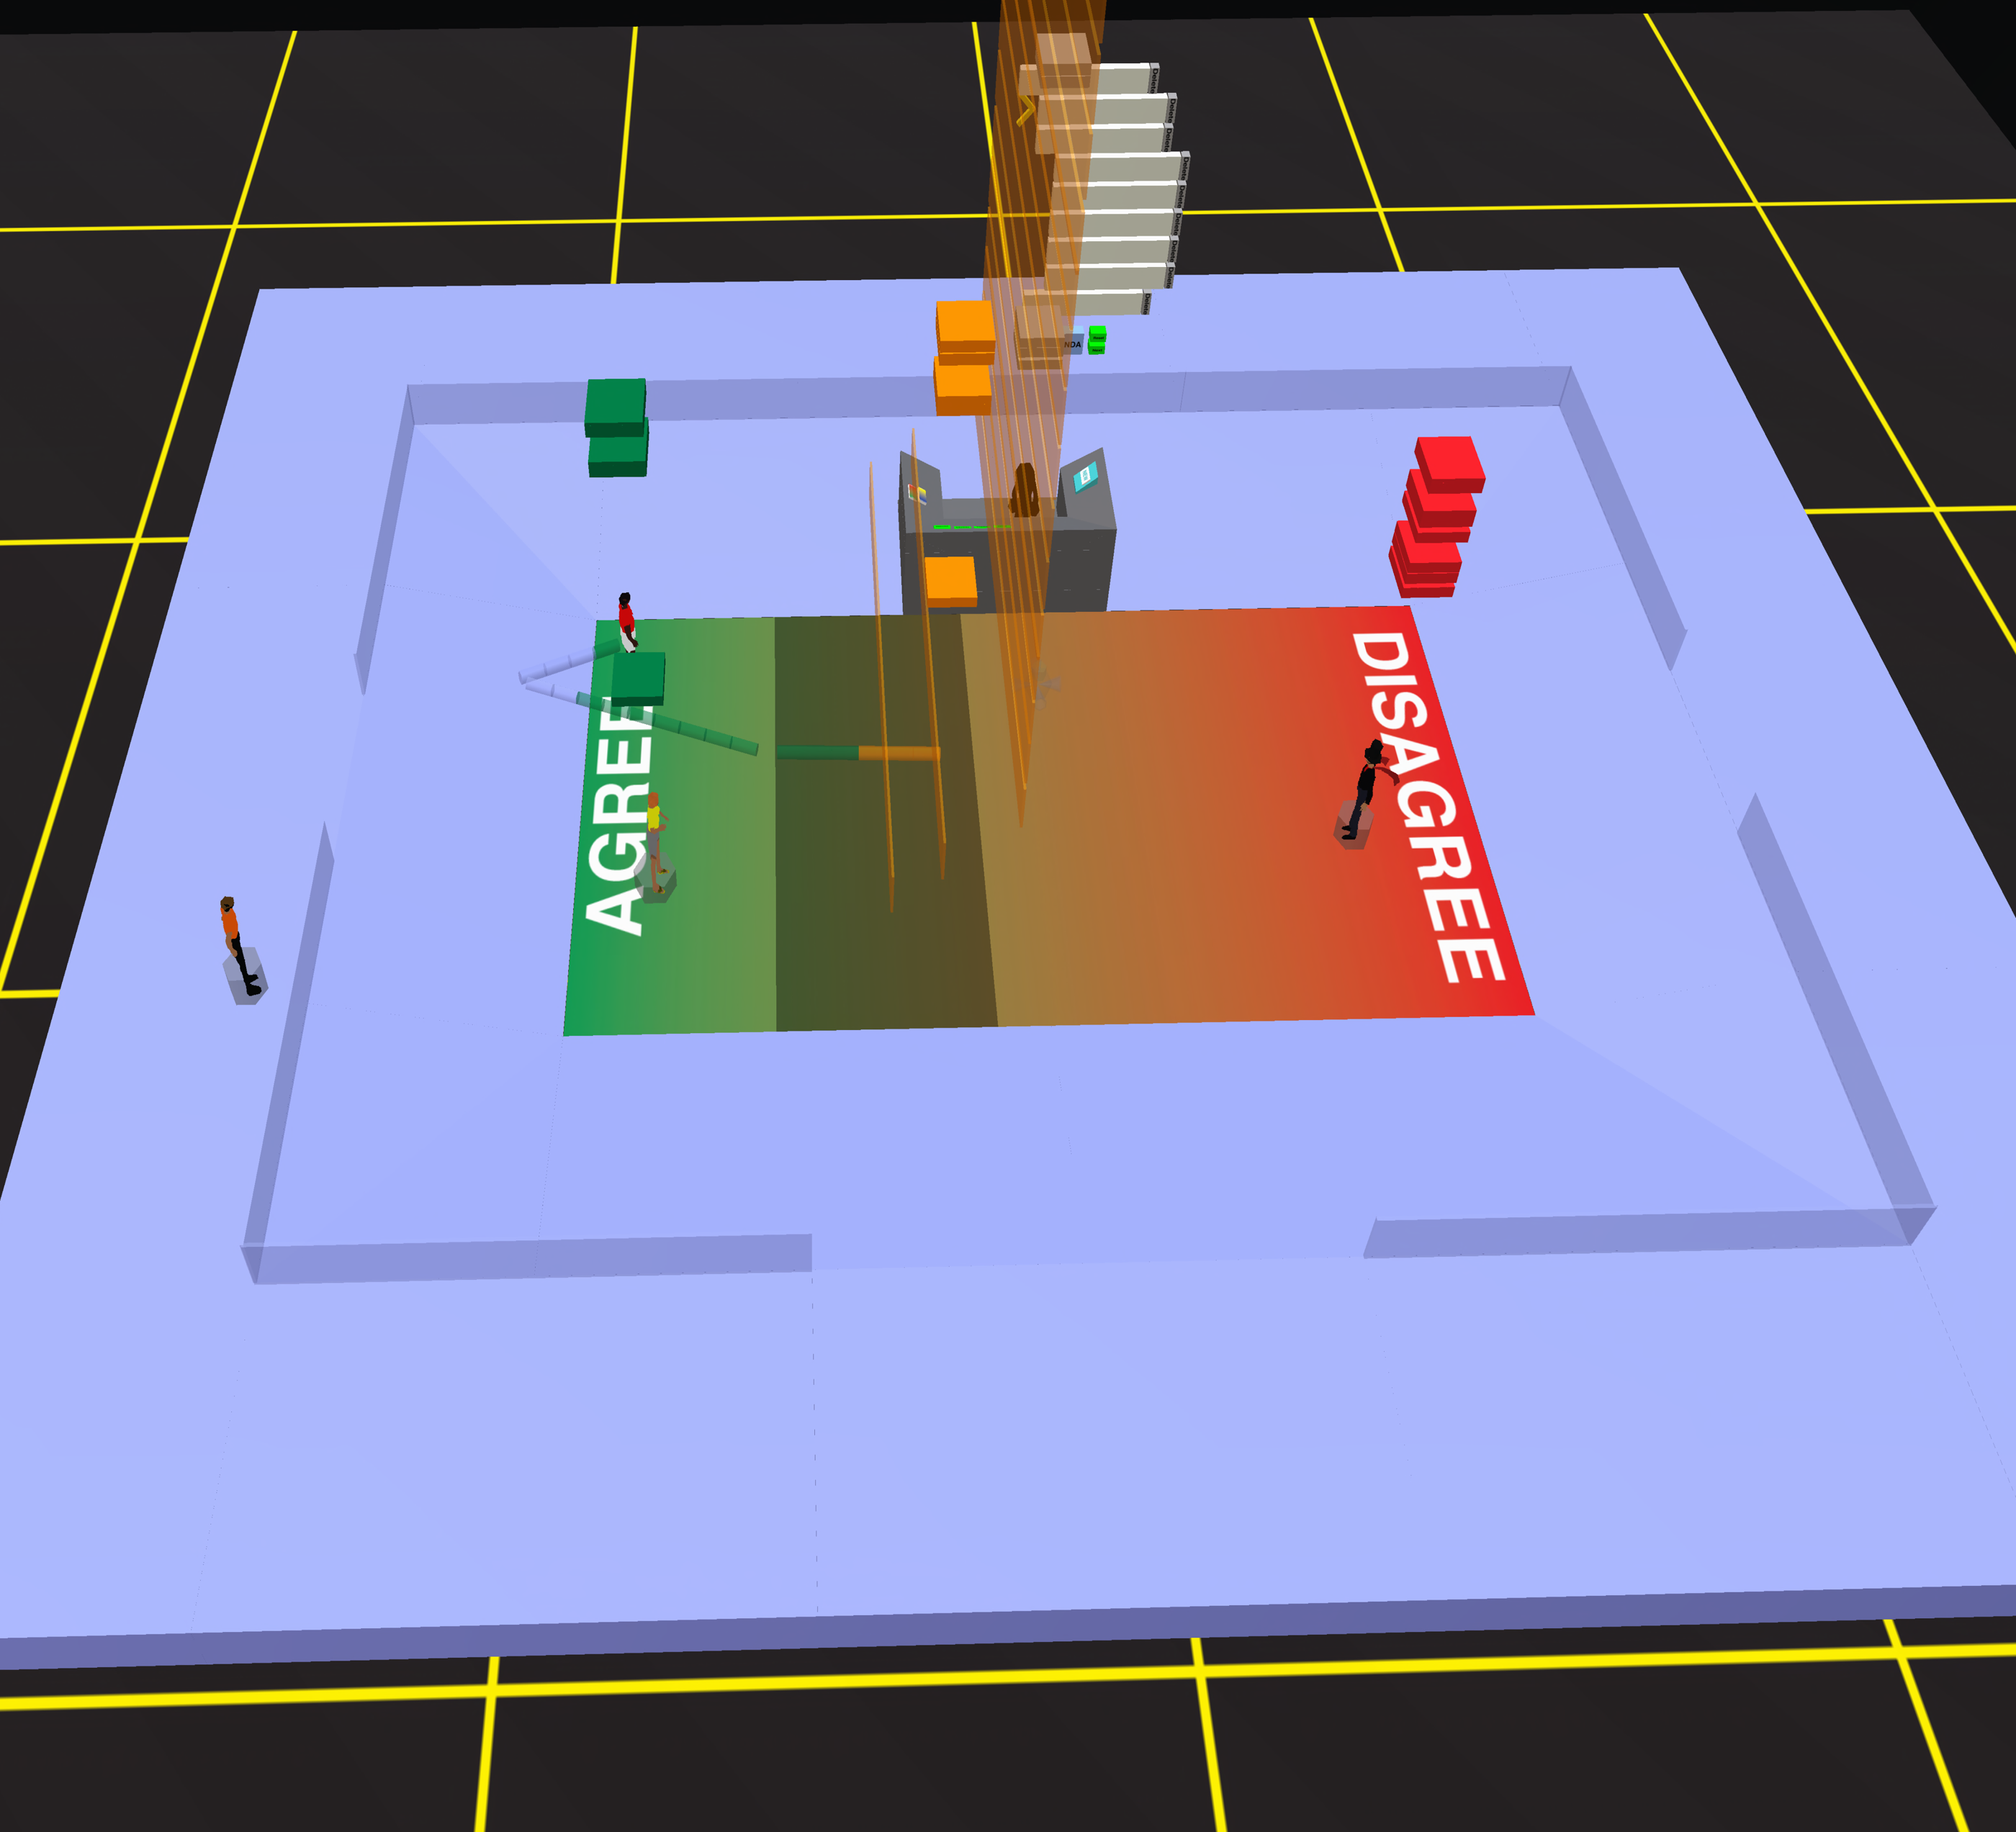
\includegraphics{figures/information-space-iso-overview.png}
	\caption{An isometric overview of the \emph{Information Space} with all the visualization components turned on.}
	\label{fig:meeting_space_overview}
\end{figure*}



\section{Presentation Spaces}


\section{Past and Future Virtuality}